
\section{CellML Adapter} % -> split into user and developer part

CellML models 

\begin{figure}%
  \centering%
  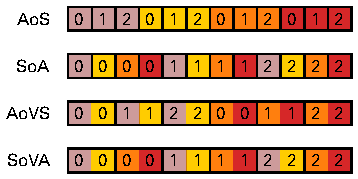
\includegraphics[width=0.6\textwidth]{images/implementation/memory_layouts.pdf}%
  \caption{Different memory layouts for the CellML model: array-of-struct (AoS), struct-of-array (SoA) and array-of-vectorized-struct (AoVS).}%
  \label{fig:memory_layouts}%
\end{figure}%

% numerous subcellular model instances solved together
% data layout AoS -> SoA

% code generator
% vectorization type simd
% type vc, explain vc and stdx::simd

% use also in fastMonodomainSolver
% GPU in FastMonodomainSolver

% ---
\newpage
\section{Solid Mechanics Solver}
% load steps, initalization in the dynamic case
% implementation of solid mechanics with analytic differentiation

\section{Mapping Between Meshes}

% mapping between meshes
% mapping between meshes, source dofs
% parallel mapping between meshes, invertability of index space represesantion

\section{Output Writers}  % move at end of usage
% output writers
% verschiedene output writer für das gleiche Faser-Modell


